\documentclass[10pt,a4paper,twocolumn]{jarticle}
%\documentclass[10pt,a4paper]{jarticle}
\usepackage{geometry}
\usepackage{pxchfon}
\usepackage{titlesec}
\usepackage{multicol}
\geometry{left=20mm,right=20mm,top=20mm,bottom=20mm}
\setlength{\columnsep}{10zw}
\usepackage{amssymb,amsmath,amsthm}
\usepackage{amsmath}
\usepackage[dvipdfmx]{graphicx}
\titleformat*{\section}{\normalsize}
\titleformat*{\subsection}{\normalsize}
\titleformat*{\subsubsection}{\normalsize}
\pagestyle{empty}
\renewcommand{\baselinestretch}{1.2}
\usepackage{multirow}
\usepackage{titlesec}
\makeatletter
\renewenvironment{thebibliography}[1]
{\section*{\refname\@mkboth{\refname}{\refname}}%
	\list{\@biblabel{\@arabic\c@enumiv}}%
	{\settowidth\labelwidth{\@biblabel{#1}}%
		\leftmargin\labelwidth
		\advance\leftmargin\labelsep
		\setlength\itemsep{0zh}%←ここの数値を調整(行間のつまり具合)
		\setlength\baselineskip{10pt}%←ここの数値を調整(追加)(文字の大きさ)
		\@openbib@code
		\usecounter{enumiv}%
		\let\p@enumiv\@empty
		\renewcommand\theenumiv{\@arabic\c@enumiv}}%
	\sloppy
	\clubpenalty4000
	\@clubpenalty\clubpenalty
	\widowpenalty4000%
	\sfcode`\.\@m}
{\def\@noitemerr
	{\@latex@warning{Empty `thebibliography' environment}}%
	\endlist}
\makeatother
\begin{document}
\twocolumn[
\begin{center}
{\large 卒業論文発表 要旨(2019年度版)\\
ワイヤレス給電システムの最適化のための能率的な動作周波数スイープ\\}
\end{center}
\begin{flushright}
	自動制御研究室\\
	森田 光流 \\
\end{flushright}
\vspace{\baselineskip}
]


\section{緒言}
ワイヤレス給電とはコネクタや金属接点の接触を用いず無線で電力を供給・伝搬することが可能な給電方法である.従来の電気製品の金属接点やコネクタを使用したものは水がかかると水による感電やショートをおこす,配線による転倒などの安全性に関して問題点がある.しかしワイヤレス給電は金属接点がないため前述の問題点を解決することができる.また非金属のものであればコイル間に存在していても送電側と受電側の電力に影響を及ぼさないため,人が立ち寄れない危険な場所や人体の中などにある機器や装置の遠隔操作ができるという点がある.(参考文献:\cite{syourai},\cite{rohm1})
\\ ワイヤレス給電の電力供給の効率の改善には色々と考えられているが本研究においては快適な周波数調整に注目し,最適動作周波数の探索することとした.最適動作周波数は電力と効率が最も大きい値を示す周波数で周波数が大きいと出力される電力が大きくなるとはかぎらない.最適動作周波数探索するためには多くの周波数を測定しなければいけないので測定時間をなるべく短くしたい.しかし,ワイヤレス給電に周波数を送った後安定な電力が出力されるまで時間がかかる.したがって本研究は測定時間と加算する周波数の大きさを調整することでそれぞれの場合において比較し最も能率的な動作周波数スイープを見つけることを目的とした.
\section{実験}
\subsection{実験回路}
\begin{figure}[h]
	\centering
	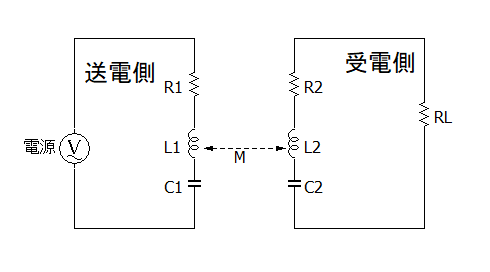
\includegraphics[scale=0.6]{wpt_2020128.png}
	\caption{ワイヤレス給電回路図}
	\label{fig:wpt_kairo}
\end{figure}
ワイヤレス給電は図\ref{fig:wpt_kairo}のように金属接点がない代わりに送電・受電にコイルを用いることにより,送電側の交流電源の電流が時間的に変化することにより受電側の磁束が変化しファラデーの電磁誘導の法則により誘導起電力が生じ誘導電流を伝えるという原理である.
なお本研究で使用した実験回路の素子の量は以下の表\ref{tab:para}ようになる.(参考文献:\cite{goizuka})
\begin{table}[h]
	\centering
	\caption{実験回路パラメータ}
	\label{tab:para}
	\begin{tabular}{|l|l|l|}
		\hline
		パラメータ                          & 記号    & 値{[}単位{]}          \\ \hline
		\multirow{2}{*}{コイルの自己インダクタンス} & $L_1$ & $23.6[\mu H]$      \\ \cline{2-3} 
		& $L_1$ & $23.6[\mu H]$      \\ \hline
		相互インダクタンス                      & $M$   & $1.98[\mu H]$      \\ \hline
		\multirow{2}{*}{コイルの内部抵抗}      & $R_1$ & 0.08{[}$\Omega${]}  \\ \cline{2-3} 
		& $R_2$ & 0.08{[}$\Omega${]} \\ \hline
		負荷抵抗                           & $R_L$ & 25{[}$\Omega${]}   \\ \hline
	\end{tabular}
\end{table}
なお,実験回路の共振周波数は以下のとおりである.
\begin{equation}
f_0=99.7kHz \nonumber
\end{equation}

\subsection{周波数スイープ}
実験による最適動作周波数を探索する方法としては周波数スイープが挙げられる.周波数スイープとは一定の時間や速度において7周波数を変化させ出力させる方法である.なお本研究における周波数スイープのやり方でする.
\begin{enumerate}
	\item  一番最初の周波数を回路に送る.なお一番最初の周波数,一番最後の周波数,1つの周波数における測定時間,次の周波数で加算する周波数(以後加算周波数)の量をあらかじめ決めておく必要がある.
	\item 決めた時間で測定する.0.1秒ずつデータが出力される.
	\item 一定時間に達したら,加算周波数を加算し一番最後の周波数に達するまで繰り返す.
\end{enumerate}
 また,先行研究ではワイヤレス給電の周波数スイープをマイコンだけで実行したが,周波数を変更するにあたってわざわざコンパイルしなければならず面倒であった.そこで本研究では周波数スイープの周波数を送る・ワイヤレス給電の電力を受け取る作業をパソコンで自動化するようにした.
\subsection{最適動作判定}
ワイヤレス給電の最適動作周波数であるには前述にも述べたが高電力・高効率であることが重要である.したがって次の計算式(\ref{eq:saiteki})を導入した.なお定数はそれぞれ周波数スイープによって出力された受電側の電力$P_2$と送電側と受電側の出力結果を使って導き出された$効率\eta$である.
\begin{equation}
(最適動作判定)=P_2\eta
\label{eq:saiteki}
\end{equation}
\subsection{能率的な周波数スイープ}
先行研究では,ひとつの周波数を送って次の周波数送るまでの測定時間を10秒だった.しかし,本研究においては多くの周波数による電圧,電流,電力を測りたいがためあまり時間をかけたくない.また加算周波数を低周波数で設定すると確かに正確に測ることが可能だが時間がかかる.また,本研究で電源の周波数を出力するためにMOSFETを使用する.MOSFETは高周波数を測定し続けると発熱し破損する恐れがある.逆に大雑把に周波数を取りすぎると正確性に欠ける.したがって周波数スイープが能率的になる周波数の測定時間と,加算周波数の量は以上のことを考慮して決めなければならない.
\subsection{シミュレーション}
実験をする前に事前にシミュレートしてみた.図\ref{fig:simudousa}はそれぞれ電力出力,効率,最適動作判定の結果である.図\ref{fig:simudousa}からわかるとおり入力する周波数が共振周波数近くのとき最適動作周波数が最大だということが分かる.
\begin{figure}[h]
	\centering
	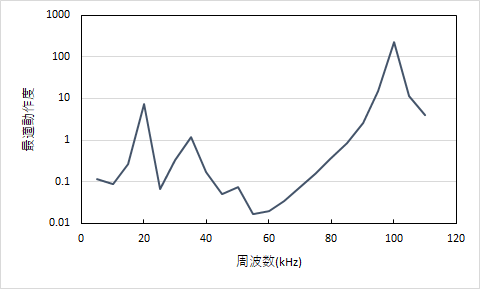
\includegraphics[scale=0.4]{saitekidousasimu.png}
	\caption{シミュレーションでの最適動作判定}
	\label{fig:simudousa}
\end{figure}
\section{実験結果・考察}
加算周波数と一つの周波数の測定時間との比較図はそれぞれ図\ref{fig:fre} 図\ref{fig:time} である.
\begin{figure}[h]
	\centering
	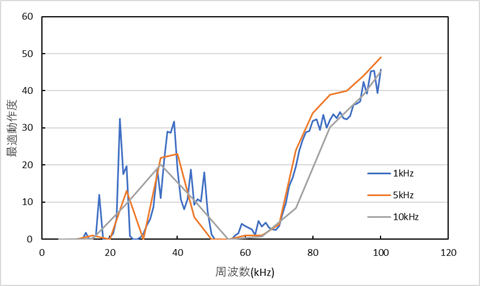
\includegraphics[scale=0.5]{hikakufre.png}
	\caption{加算周波数の比較}
	\label{fig:fre}
\end{figure}
\begin{figure}[h]
	\centering
	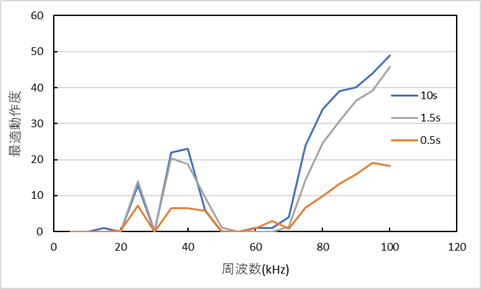
\includegraphics[scale=0.5]{hikakutime.png}
	\caption{一つの周波数につきの測定時間の比較}
	\label{fig:time}
\end{figure}
図\ref{fig:fre} の加算周波数はそれぞれ$1kHz,5kHz,10kHz$で動作周波数スイープしたときである.計測時間はどの加算周波数においても10秒と設定した.図\ref{fig:fre} にもわかる通り$10kHz$のときは測定時間が短縮化されたが加算する範囲が大きすぎるため,$10kHz$間の出力変化に対応できない.また,加算周波数が$1kHz$のように低周波数ならば全体の測定時間が長くなる.また上にも述べた通りMOSFETの破損の原因に繋がる.したがって5kHzの時は10kHz間の出力変化に対応できかつ測定時間を短くすることができるので加算周波数では5kHzのときが最も能率的である.\\ 図\ref{fig:time} はそれぞれ0.5秒,1.5秒,10秒のときを計測した場合である.また加算周波数はどの場合において$5kHz$なお本研究はそれ以外の時間も計測したが代表として3つ上げる.0.5秒のときまだ電力が出力されていないので小さい値で出力される.よって,10秒のときと比べて最も近い値が出力された1.5秒の時が測定時間に最適な時間である.
\begin{figure}[h]
	\centering
	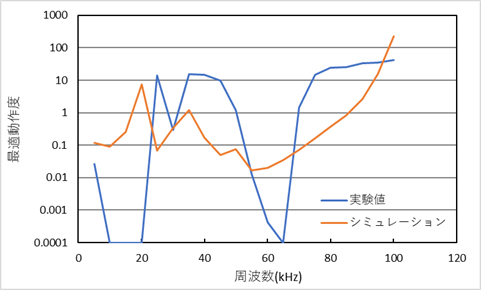
\includegraphics[scale=0.4]{simuhikaku.png}
	\caption{シミュレーションと実験結果との比較}
	\label{fig:simu-zitu}
\end{figure}
\\ それぞれ決定された周波数を下にシミュレーションと比較すると.図\ref{fig:simu-zitu} のようになる.
図\ref{fig:simu-zitu}からわかる通り出力結果にずれが生じていることが分かる.これは実験素子の実際の値が表\ref{tab:para}と比べてそれぞれ自己相互インダクタンス,コイルの内部抵抗,送電側受電側のコンデンサのずれが生じているから回路の共振周波数が変わりその結果電力の出力にずれが生じていると考えられる.

\section{今後の方針}
能率的な周波数スイープを使うことにより,測定時間最短化することができた.それにより時間最短化することにより,ワイヤレス給電の状況によって周波数を変化させることにより受電側どんな状況にあってもいつも高電力を出力するように制御するということができると考えられる.しかし,ワイヤレス給電の電力出力を自動制御するには1.5秒でも遅い.ワイヤレス給電のさらに正確かつさらに最短な能率的周波数スイープさせる方法・回路中のローパスフィルタの時定数見直しが求められる.また,低い電圧どおしで乗算器に通すと性能上うまく出力されない問題があるので乗算器またはオペアンプの見直しも求められる.
\begin{thebibliography}{50}
	\bibitem{rohm1}ローム株式会社:”ワイヤレス給電とは”ーエレクトロニクス豆知識, https://www.rohm.co.jp/electronics-basics/wireless-charging/wireless-charging\_what1,最終アクセス:2020/1/20
	\bibitem{goizuka}五位塚潤:"低周波数域駆動によるワイヤレス給電回路", 宮崎大学学士論文, 平成29年度
	\bibitem{syourai}B\&PLUS:"ワイヤレス給電の現状と未来",https://www.b-plus-kk.jp/about/mechanism.html 最終アクセス:2020/1/23
\end{thebibliography}
\end{document}
